\section{Klassifizierungsgenauigkeit der Standorte}
Die Klassifizierungsgenauigkeit der ML-Modelle zur Standortbestimmung wurde mit verschiedenen Konfigurationen über komplexer werdende Datenmengen evaluiert.
In Kapitel \ref{sec:model_dt} und Kapitel \ref{sec:model_ffnn} werden die einzelnen Konfigurationen der ML-Modelle beschrieben.
Die Komplexität wird über die Anzahl der Standorte definiert.
Um die Standortkomplexität zu erhöhen, wurden die Datenmengen um weitere Routen erweitert.
Dies impliziert aber, dass die Testmengen nicht unter den verschiedenen Standortkomplexitäten vergleichbar sind, da mit jeder Route die Testmenge erweitert wird.
Die berechneten Klassifizierungswahrscheinlichkeiten sind jeweils der Durchschnitt der Klassifizierungswahrscheinlichkeiten aller Routen in der Testmenge.
\newline
\newline
Außerdem unterscheiden sich die Kodierungsansätze, je nach Standortkomplexität.
Für die Standortkomplexitäten 9, 17, 25 und 52 wurde der Kodierungsansatz verwendet, bei denen nur die Knoten und ein zusätzlicher unbekannter Standort betrachtet wird.
Für die Standortkomplexitäten 16, 32, 48 und 102 wurde der Kodierungsansatz verwendet, bei denen Knoten und Kanten betrachtet werden.
Ein besserer Ansatz, um Daten mit beliebiger Komplexität zu generieren wird in Kapitel \ref{chapter:discussion} diskutiert.
\newline
\newline
Mian hat die Klassifizierungsgenauigkeit $P(A)_{\text{cont}}$ betrachtet.
Er konnte mit einem WFFNN (Windowed FFNN) bei einer Route mit drei Pfaden und 14 Standorten eine Klassifizierungsgenauigkeit von 94,1\% erreichen \cite{naveedThesis}.
Abbildung \ref{fig:best_dt_acc_vs_knn_using_cont} vergleicht $P(A)_{\text{cont}}$ der Entscheidungsbaum basierten Klassifizierer und FFNN über verschiedene Standortkomplexitäten.
Dabei wurde stets die höchste Klassifizierungsgenauigkeiten aller evaluierten Konfigurationen ausgewählt.
\begin{figure}[h!]
    \centering
    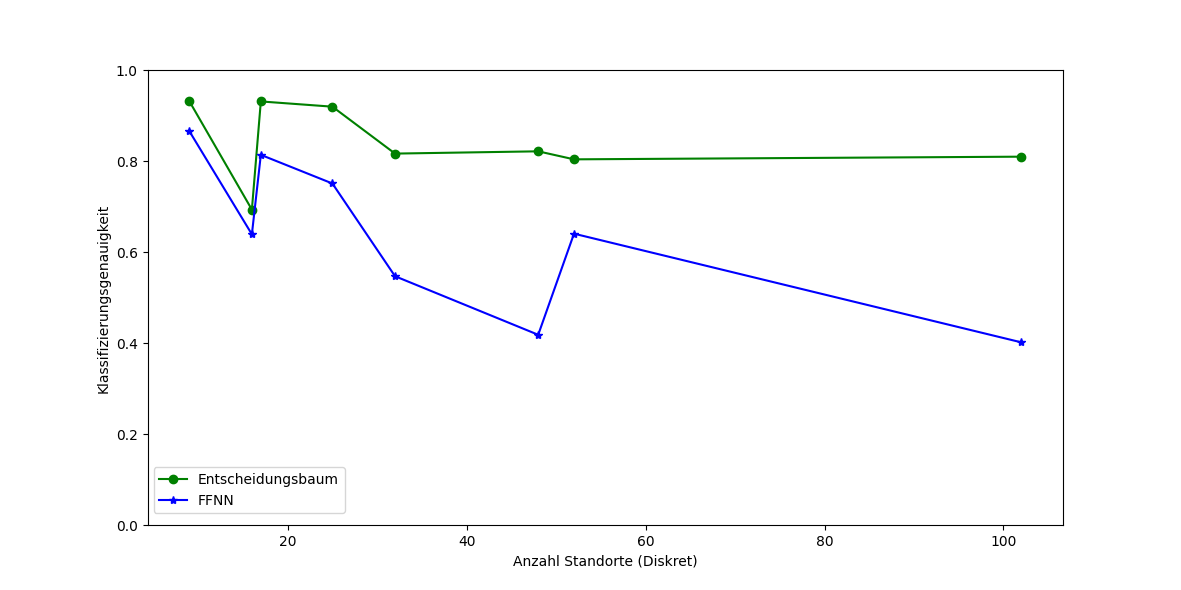
\includegraphics[width=\linewidth]{images/best_dt_vs_best_ffnn_over_num_loc_using_acc_cont.png}
    \caption{Die besten Klassifizierungsgenauigkeiten $P(A)_{\text{cont}}$ über Standortkomplexitäten.}
    \label{fig:best_dt_acc_vs_knn_using_cont}
\end{figure}
\newline
\newline
Mian kodierte in seinem Ansatz die Kanten als Standorte, was sich von den in dieser Arbeit benutzten Ansätzen unterscheidet.
Die in dieser Arbeit evaluierten Standortkomplexitäten, die Mians Evaluation am nächsten kommen, sind 16, mit dem Kodierungsansatz, der Kanten und Knoten kodiert,
und 17, mit dem Kodierungsansatz, der nur Knoten kodiert.
\newline
\newline
Aus Tabelle \ref{tab:predictions_by_acc_cont} können die Klassifizierungsergebnisse dieser Standortkomplexitäten entnommen werden.
Der beste Entscheidungswald mit einer Standortkomplexität von 16 hat eine Klassifizierungsgenauigkeit $P(A)_{\text{cont}}$ von 83,52\%.
Das ist 10,27 Prozentpunkte schlechter als Mians Ansatz.
Das beste FFNN ist 30,16 Prozentpunkte schlechter.
\newpage
Der beste Entscheidungswald mit einer Standortkomplexität von 17 ist 0,31 Prozentpunkte besser als Mians Ansatz.
Das beste FFNN ist 6,88 Prozentpunkte schlechter.
Anzumerken ist aber, dass die Standortkomplexität höher ist und ein deutlich kleineres Datenfenster verwendet wurde,
um die Feature-Menge zu generieren, wodurch die resultierenden ML-Modelle kleiner sind.
\newline
\newline
ML-Modelle sind besser vergleichbar, wenn toleriert wird, dass das ML-Modell den Standort etwas zu früh betritt oder etwas zu spät verlässt,
solange es kontinuierlich den selben Standort angibt, da bei den Übergängen zwischen Standorten nicht immer eindeutig ein Standort bestimmt werden kann.
Tabelle \ref{tab:predictions_by_acc_5_cont} gibt diese Klassifizierierungsgenauigkeit $P(B\leq5)$ an, wobei bis zu 5 Klassifizierungen toleriert werden.
\begin{table}[h!]
    \hspace{-2cm}
    \begin{tabular}{ | c | c | c | c | c | c | c | c | c | c | }
        \hline
        \multicolumn{2}{ | l |}{$P(B=5)_{\text{cont}}$ über Standorte} & 9 & 16 & 17 & 25 & 32 & 48 & 52 & 102 \\\hline
        \multicolumn{10}{| l |}{\textbf{Entscheidungswälder}}\\\hline
        Waldgröße & Max. Baumgröße & \multicolumn{8}{ c |}{}\\\hline
        16 & 8 & 98.24\% & 78.83\% & 97.98\% & 94.30\% & 82.18\% & 82.53\% & 80.22\% & 78.17\% \\\hline
        16 & 16 & 97.07\% & 73.68\% & 97.66\% & 95.32\% & 89.54\% & 87.10\% & 82.73\% & 87.77\% \\\hline
        16 & 32 & 97.91\% & 74.03\% & 97.42\% & 96.19\% & 85.19\% & 85.39\% & 85.70\% & 84.15\% \\\hline
        16 & 64 & 97.91\% & 74.03\% & 97.42\% & 96.19\% & 85.19\% & 85.39\% & 85.70\% & 84.15\% \\\hline
        8 & 32 & 96.73\% & 89.49\% & 98.35\% & 96.39\% & 88.34\% & 89.32\% & 89.60\% & 83.67\% \\\hline
        32 & 32 & 97.84\% & 74.58\% & 98.64\% & 95.85\% & 87.38\% & 86.47\% & 85.37\% & 85.38\% \\\hline
        64 & 32 & 98.11\% & 80.29\% & 98.42\% & 95.35\% & 87.93\% & 87.68\% & 84.17\% & 86.16\% \\\hline
        32 & 64 & 97.84\% & 74.58\% & 98.64\% & 95.85\% & 87.38\% & 86.47\% & 85.37\% & 85.38\% \\\hline
        \multicolumn{10}{| l |}{\textbf{Feed Forward neuronale Netzwerke}}\\\hline
        \#Schichten & \#Neuronen & \multicolumn{8}{ c |}{}\\\hline
        1 & 16 & 96.11\% & 71.77\% & 89.37\% & 77.19\% & 43.45\% & 45.03\% & 71.55\% & 40.74\% \\\hline
        1 & 32 & 94.59\% & 72.18\% & 88.82\% & 80.91\% & 60.22\% & 45.08\% & 70.47\% & 43.07\% \\\hline
        1 & 64 & 92.71\% & 63.21\% & 90.18\% & 84.11\% & 48.12\% & 38.78\% & 72.33\% & 32.70\% \\\hline
        1 & 128 & 95.50\% & 69.99\% & 93.33\% & 83.66\% & 49.63\% & 31.27\% & 75.39\% & 41.06\% \\\hline
        2 & 32 & 96.17\% & 57.58\% & 88.34\% & 80.28\% & 65.24\% & 33.54\% & 70.91\% & 34.12\% \\\hline
        4 & 32 & 90.45\% & 66.50\% & 85.20\% & 76.55\% & 46.81\% & 26.17\% & 67.56\% & 36.70\% \\\hline
        8 & 32 & 88.06\% & 57.44\% & 86.54\% & 78.26\% & 34.54\% & 34.35\% & 70.57\% & 48.82\% \\\hline
        4 & 64 & 90.98\% & 62.21\% & 86.66\% & 81.08\% & 51.40\% & 22.54\% & 70.94\% & 45.54\% \\\hline
    \end{tabular}
    \caption{$P(B\leq5)_{\text{cont}}$ über Standorte und Konfigurationen der ML-Modelle.}
    \label{tab:predictions_by_acc_5_cont}
\end{table}
\newline
\newline
Der Entscheidungsbaum basierte Klassifizierer skaliert sehr gut mit der steigenden Standortkomplexität.
Im Schnitt fällt die Klassifizierungsgenauigkeit um 0,16 Prozentpunkte pro zusätzlichen Standort.
Bei einer Standortkomplexität von 102 wird immer noch eine Klassifizierungsgenauigkeit $P(B\leq5)_{\text{cont}}$ von 87,77\% erreicht.
Als beste maximale Baumhöhe hat sich 16 herausgestellt, wobei 32 und 64 marginal schlechtere Ergebnisse erzielten.
Eine maximale Baumhöhe von 8 war nicht ausreichend, da es für hohe Standortkomplexitäten schlechtere Ergebnisse erzielt hat.
Bei gleicher Waldgröße haben die maximalen Baumhöhen von 32 und 64 equivalente Ergebnisse erzielt,
d. h. für die evaluierten Szenarien wird nicht mehr als eine maximale Baumhöhe von 32 benötigt.
\newpage
Dies schließt aber nicht aus, dass andere Szenarien nicht von größeren maximalen Baumhöhen profitieren könnten.
Die verschiedenen Waldgrößen unterscheiden sich nicht stark.
Eine Waldgröße von 8 hat nur marginal schlechtere Ergebnisse bei 102 Standorten erzielt, als die Waldgrößen 16, 32 und 64.
Aus diesem Grund ist eine Waldgröße von 8 ausreichend, oder könnte womöglich reduziert werden.
\newpage
Die evaluierten FFNNs skalieren mit steigender Standortkomplexität deutlich schlechter als die Entscheidungswälder.
Im Schnitt fällt die Klassifizierungsgenauigkeit um 0,51 Prozentpunkte pro zusätzlichen Standort.
Auffallend ist, dass die Klassifizierungsergebnisse bei FFNNs mit dem Kodierungsansatz, in dem Kanten und Knoten kodiert werden,
deutlich schlechter sind als beim Kodierungsansatz, in dem nur die Knoten kodiert werden.
Wenn man nur den letzteren Kodierungsansatz betrachtet, fällt die Klassifizierungsgenauigkeit im Schnitt nur um 0,22 Prozentpunkte pro zusätzlichen Standort.
Aus den Daten ist nicht zu schließen, wie sich die Anzahl der Schichten und Neuronen pro Schicht auf die Klassifizierungsgenauigkeit auswirken.
Große FFNNs sind im Vergleich zu kleinen FFNNs aber sehr volatil in der Klassifizierungsgenauigkeit.
\newline
\newline
Sowohl bei den Entscheidungswäldern, als auch bei den FFNNs, ist eine geringere Klassifizierungsgenauigkeit mit dem Kodierungsansatz, der Kanten und Knoten kodiert,
zu beobachten, als mit dem Kodierungsansatz, der nur die Knoten kodiert.
Insbesondere zwischen den Standortkomplexitäten 16 und 17, sowie 32, 48 und 52 ist diese Diskrepanz zu erkennen.
Aus diesem Grund ist zu schließen, dass der Kodierungsansatz, der nur Knoten kodiert, besser skaliert, als der Kodierungsansatz, der Kanten und Knoten kodiert.